\section{Empirical evaluation of least squares}

I implemented the Ho-Kalman algorithm
and the least-squares methods from \cite{oymak2019singletraj}
and \cite{simchowitz2019parametric},
along with the simple averaging mentioned
in the introduction of \cite{oymak2019singletraj}.
The least squares method from \cite{oymak2019singletraj} computes
\[ \hat G = \arg\min_G \Verts{G \overline{U} - Y}_F^2 \]
where $Y$ is a matrix whose $t$th column is $y_t$
and $\overline U$ is a matrix whose $t$th column is
$[u_t^\top, u_{t-1}^\top, \ldots, u_{t-T+1}^\top]^\top$.

The least squares method from \cite{oymak2019singletraj} uses two steps:
\begin{align*}
\phi &= \arg\min_\varphi \Verts{\varphi K - Y}_F^2 + \mu \Verts{\varphi}_F^2 \\
\hat G &= \arg\min_G \Verts{G \overline{U} - (Y - \phi K)}_F^2
\end{align*}
where $K$ is a matrix whose $t$th column is
$[y_{t-T}^\top, y_{t-2T}^\top, \ldots, y_{t-LT}^\top]^\top$
for some fixed constant $L$.

In each experiment, I produced synthetic systems
in a manner similar to \cite{oymak2019singletraj}.
I used a state space of $\Real^5$ (i.e. $n = 5$),
an input space of $\Real^3$ (i.e. $p = 3$),
and an observation space of $\Real^2$ (i.e. $m = 2$).
The matrix $A$ has normally distributed entries
with mean $0$ and variance $1$,
but is rescaled so that $\rho(A)$ is some desired value.
The matrix $A$ has normally distributed entries
with mean $0$ and variance $1/n$,
and the matrices $C$ and $D$ have normally distributed entries
with mean $0$ and variance $1/m$.
I simulated the systems with initial condition $x_1 = 0$
and $u_t \sim \mathcal N(0, \sigma_u^2 I)$,
where $\sigma_u = 1$ and $\sigma_w = \sigma_z = 1/4$.
In all of the experiments
except the one about the performance of Ho-Kalman,
I set $T = 18$.
My code is available at
{\tt https://github.com/bnjw5jhyxn/ese618\_project\_code}.

\begin{figure}
\includegraphics[scale=0.7]{ho_kalman}
\end{figure}
When I evaluated the performance of Ho-Kalman,
I computed $\hat G$
by running the Ho-Kalman algorithm on $G$
(the true Markov parameters),
then using $\hat A$, $\hat B$, and $\hat C$
to reconstruct the Markon parameters.
The performance of the Ho-Kalman algorithm
degrades when the system is unstable
because the Markov parameters blow up.
Since this effect is exaggerated
as you compute more Markov parameters,
I set $T_1 = 45$ and $T_2 = 40$ in this figure.
This degredation doesn't matter very much
in our setting since we don't run our experiments
with a stabilizing controller
and thus our state blows up anyway for unstable systems,
so we can't collect data with the current experimental setup.

\begin{figure}
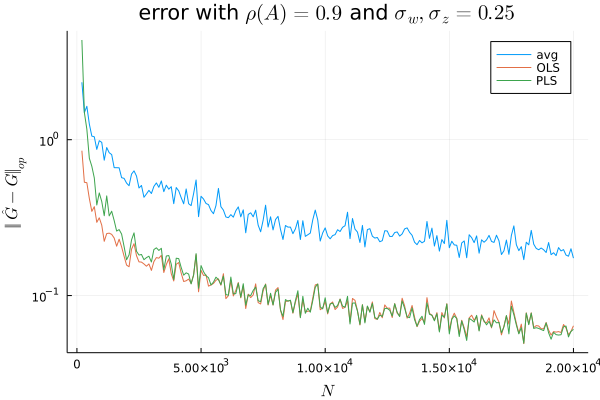
\includegraphics[scale=0.7]{rho_small}
\end{figure}
In the regime where $\rho(A) \ll 1$,
averaging is worse than the other two methods.
The prefiltered least squares by \cite{simchowitz2019parametric}
is worse at small sample sizes because
it gives up the first few samples in order to learn a filter
that subtracts out the correlations of $y_t$
with $y_0, \ldots, y_{t-T}$.
This filter is useless here because the correlation is negligible,
and prefiltered least squares is identical to
the ordinary least squares by \cite{oymak2019singletraj},
but with fewer samples.

\begin{figure}
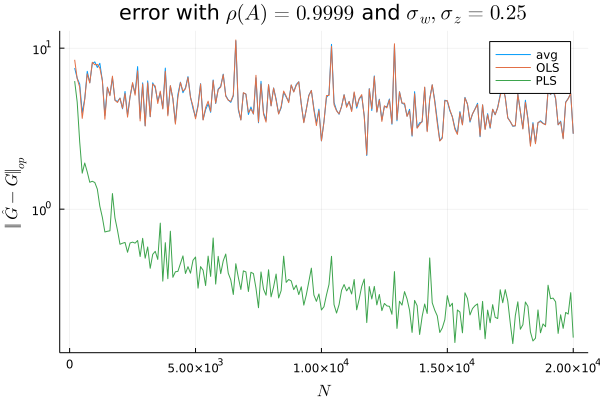
\includegraphics[scale=0.7]{rho_1me}
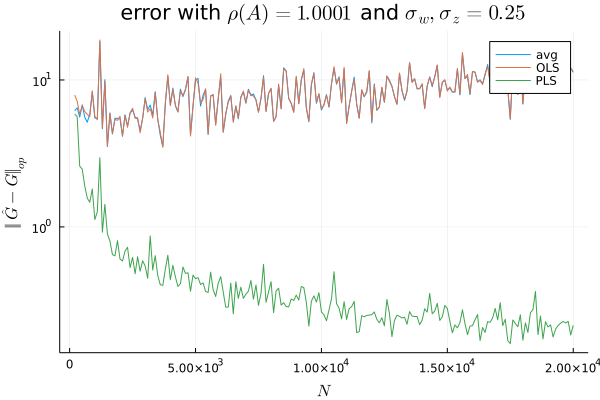
\includegraphics[scale=0.7]{rho_1pe}
\end{figure}
In the regime where $\rho(A) \approx 1$,
prefiltered least squares continues to perform well, as expected,
and the performance of ordinary least squares
degrades to the level of simple averaging.

\begin{figure}
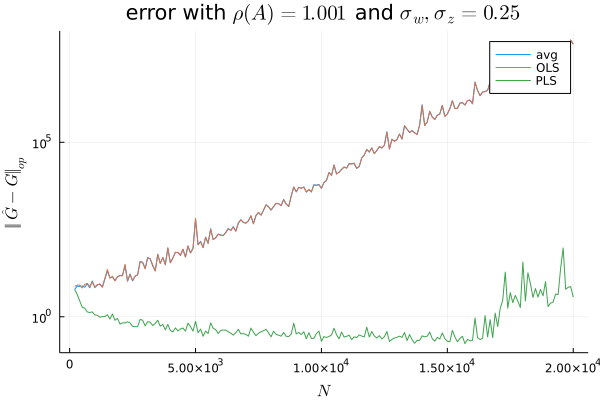
\includegraphics[scale=0.7]{rho_big}
\end{figure}
As $\rho(A)$ gets bigger, averaging and ordinary least squares
become basically useless
and actually produce worse estimates as they get more data,
since the data points are strongly correlated.
Prefiltered least squares continues to be reasonable
with small amounts of data,
but the system eventually blows up so much
that the signal from the recent timesteps
gets drowned out by the noise from the timesteps
far in the past, causing prefiltered least squares to break down.

\begin{figure}
\includegraphics[scale=0.7]{baseline_stability}
\end{figure}

\begin{figure}
\includegraphics[scale=0.7]{averaging_convergence}
\end{figure}
Letting $\hat G_{\text{avg}}$ denote the estimate of $G$ using averaging,
and letting $\hat G_{\text{ols}}$ denote the estimate
using ordinary least squares,
we can explain the performance of averaging by observing that
$\hat G_{\text{avg}} - G
= (\hat G_{\text{avg}} - \hat G_{\text{ols}}) + (\hat G_{\text{ols}} - G)$.
All three of these quantities converge to $0$
as the amount of data increases,
with the convergence of $\hat G_{\text{ols}} - G$
becoming slower as $\rho(A)$ approaches $1$,
as analyzed by \cite{oymak2019singletraj}.

We can better understand the convergence of
$\hat G_{\text{avg}} - \hat G_{\text{ols}}$ to $0$ by observing that
\begin{align*}
\hat G_{\text{avg}} - \hat G_{\text{ols}}
&= \frac{1}{N \sigma_u^2} Y \overline{U}^\top - \hat G_{\text{ols}} \\
&= \frac{1}{N \sigma_u^2} Y \overline{U}^+ \overline{U} \overline{U}^\top - \hat G_{\text{ols}} \\
&= \hat G_{\text{ols}} \parens{\frac{1}{N \sigma_u^2} \overline{U} \overline{U}^\top} - \hat G_{\text{ols}} \\
&= \hat G_{\text{ols}} \parens{\frac{1}{N \sigma_u^2} \overline{U} \overline{U}^\top - I}, \\
\end{align*}
where $\overline{U}^+$ is the Moore-Penrose inverse of $\overline{U}$.
Since the entries of $\overline{U}$ are Gaussians
with mean $0$ and variance $\sigma_u^2$,
we can see that the diagonal entries of
$\frac{1}{N \sigma_u^2} \overline{U} \overline{U}^\top$
are of the form $\frac{1}{N} \sum _{i=1} ^N \parens{\frac{x_i}{\sigma_u}}^2$,
where the $x_i$'s are i.i.d.~Gaussians with mean $0$ and variance $\sigma_u^2$.
The diagonal entries thus concentrate around $1$.
The off-diagonal entries
are of the form $\frac{1}{N} \sum _{i=1} ^N \parens{\frac{x_{i,1}}{\sigma_u}}
\parens{\frac{x_{i,2}}{\sigma_u}}$,
where the $x_{i,j}$'s are Gaussians with mean $0$ and variance $\sigma_u^2$,
and where $x_{i,1}$ is independent of $x_{i,2}$.
The off-diagonal entries thus concentrate around $0$.
Thus, $\frac{1}{N \sigma_u^2} \overline{U} \overline{U}^\top$ converges to $I$
and this convergence does not depend on the stability properties of the system.
Since $\hat G_{\text{ols}}$ doesn't blow up as we get more data,
it follows that $\hat G_{\text{avg}} - \hat G_{\text{ols}}$ converges to $0$
and that its convergence does not depend on the stability of the system.

We can therefore conclude that when $\rho(A)$ is far from $1$,
the convergence of $\hat G_{\text{ols}} - G$ is faster
than the convergence of $\hat G_{\text{avg}} - \hat G_{\text{ols}}$,
so ordinary least squares has much smaller error than averaging.
When $\rho(A)$ is close to $1$, on the other hand,
the convergence of $\hat G_{\text{ols}} - G$ is slower
and the difference between
$\hat G_{\text{avg}}$ and $\hat G_{\text{ols}}$ is negligible
compared to the difference between $\hat G_{\text{ols}}$ and $G$.
